\documentclass[10pt]{article}

%\usepackage{amsfonts, amsthm, amsmath, enumerate, tikz, fullpage}
\usepackage{amsfonts, amsthm, amsmath, enumerate}

\newcommand{\card}[1]{\left| #1 \right|}
\newcommand{\brackets}[1]{\left< #1 \right>}
\newcommand{\nat}{\mathbb{N}}
\newcommand{\ints}{\mathbb{Z}}
\newcommand{\reals}{\mathbb{R}}
\newcommand{\chtitle}[1]{\noindent \vspace{5mm}\textbf{Chapter #1}\vspace{3mm}}

\begin{document}
\begin{flushleft}
\textbf{\noindent
STUDENT NAME - EID\\
CS 341 Automata Theory \\
Homework 15 \\
Due: Tuesday, April 30}\\
\end{flushleft}

\noindent
This assignment covers Chapters 22 and 24.\\

\begin{enumerate}[1)]

% ---
% 1
% ---

\item
Solve the linear Diophantine farmer problem presented in Section 22.1.
\begin{proof}[Solution]
\end{proof}

%---
% 2
%---

\item
Consider the following instance of the Post Correspondence problem.  Does it have a solution?  If so, show one.\\

//TODO: Table width

\begin{tabular}{| l | l | l |}
  \hline
  &X&Y\\
  \hline
  1&\texttt{a}&\texttt{bab}\\
  \hline
  2&\texttt{bbb}&\texttt{bb}\\
  \hline
  3&\texttt{aab}&\texttt{ab}\\
  \hline
  4&\texttt{b}&\texttt{a}\\
  \hline
\end{tabular}
\begin{proof}[Solution]
\end{proof}

% ---
% 3
% ---

\item
Prove that, if an instance of the Post Correspondence problem has a solution, it has an infinite number of solutions. (Hint: this is really easy.)
\begin{proof}[Proof]
\end{proof}

% ---
% 4
% ---

\item
) Let $TILES = \{\brackets{T}$ : any finite surface on the plane can be tiled, according to the rules described in the book, with the tile set $T$\}.  Let $s$ be the string that encodes the following tile set:\\

//TODO: include graphics\\

Is $s \in TILES$?  Prove your answer.
\begin{proof}[Answer]
\end{proof}
\begin{proof}[Proof]
\end{proof}

% ---
% 5
% ---

\item
Is $L = \{\brackets{M}$ : $M$ is a PDA and $L(M) = \{x\ :\ x \in \{a, b\}^*$ and $\exists m\ (\card{x} = 2^m)\}\}$ decidable?  Prove your answer.
\begin{proof}[Answer]
\end{proof}
\begin{proof}[Proof]
\end{proof}

% ---
% 6
% ---

\item
A language $L$ is \textbf{D-complete} iff (1)  $L$ is in $D$, and (2) for every language  $L'$ in $D$,  $L' \leq _M L$.  Consider the following claim: If $L \in D$ and $L \neq \Sigma ^*$ and $L \neq \emptyset$, then $L$ is D-complete.  Prove or disprove this claim.
\begin{proof}[Proof]
\end{proof}

% ---
% 7
% ---

\item
Let $\Sigma = \{1\}$.  Show that there exists at least one undecidable language with alphabet $\Sigma$.   (Hint: Use a counting argument.)
\begin{proof}[Proof]
\end{proof}

% ---
% 8 
% ---

\item
The following sequence of figures corresponds to a fractal called a \textit{Koch island}:\\

%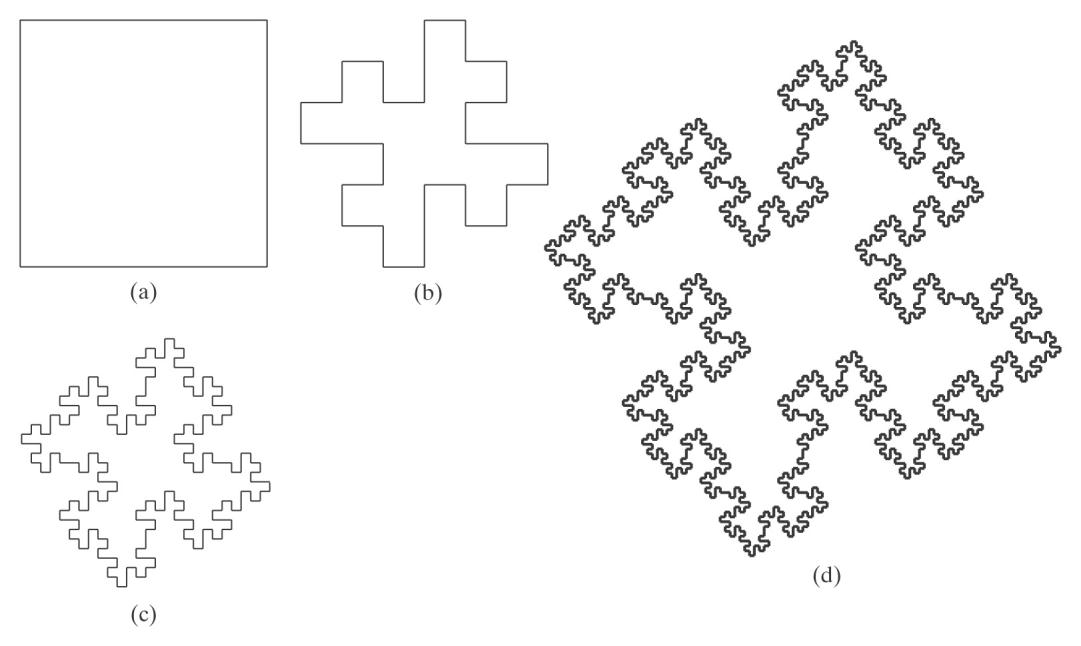
\includegraphics[scale=.2]{/images/p8.png}

These figures were drawn by interpreting strings as turtle programs, just as we did in Example 24.5 and Example 24.6.  The strings were generated by an L-system $G$, defined with:

\begin{align*}
\Sigma &= \{F, +, -\}.\\
\omega &= F - F - F - F
\end{align*}

To interpret the strings as turtle programs, attach meanings to the symbols in $\Sigma$ as follows (assuming that some value for $k$ has been chosen):
\begin{itemize}
\item
$F$ means move forward, drawing a line of length $k$.
\item
$+$ means turn left $90^\circ$.
\item
$-$ means turn right $90^\circ$.
\end{itemize}

Figure (a) was drawn by the first generation string $\omega$.  Figure (b) was drawn by the second generation string, and so forth.  $R_G$ contains a single rule.  What is it?
\begin{proof}[Answer]
\end{proof}
\end{enumerate}
\end{document}
